\apendice{Especificación de Requisitos}

\section{Introducción}

\section{Objetivos generales}

\section{Catálogo de requisitos}

\section{Prototipado}
\label{s:mockups}

Como es conocido, en el mundo del desarrollo \textit{software} suele haber una diferencia en el entendimiento de una aplicación por parte del cliente y del equipo de desarrollo que puede desembocar en malentendidos que causen retrasos temporales y pérdidas económicas.

Con el fin de reducir dichas desventajas y realizar un diseño que se adapte a los requerimientos del usuario, se ha decidido realizar una fase de prototipado durante las entrevistas del producto. Esto ha permitido identificar posibles diferencias entre el equipo del desarrollo y el cliente (representado por el \textit{product owner}), facilitando la comunicación y colaboración entre ambas partes.

Se adjuntan a continuación los diferentes \textit{mockups} realizados durante esta fase.


\begin{figure}[h]
	\caption{Prototipos: página principal}
	\centering
	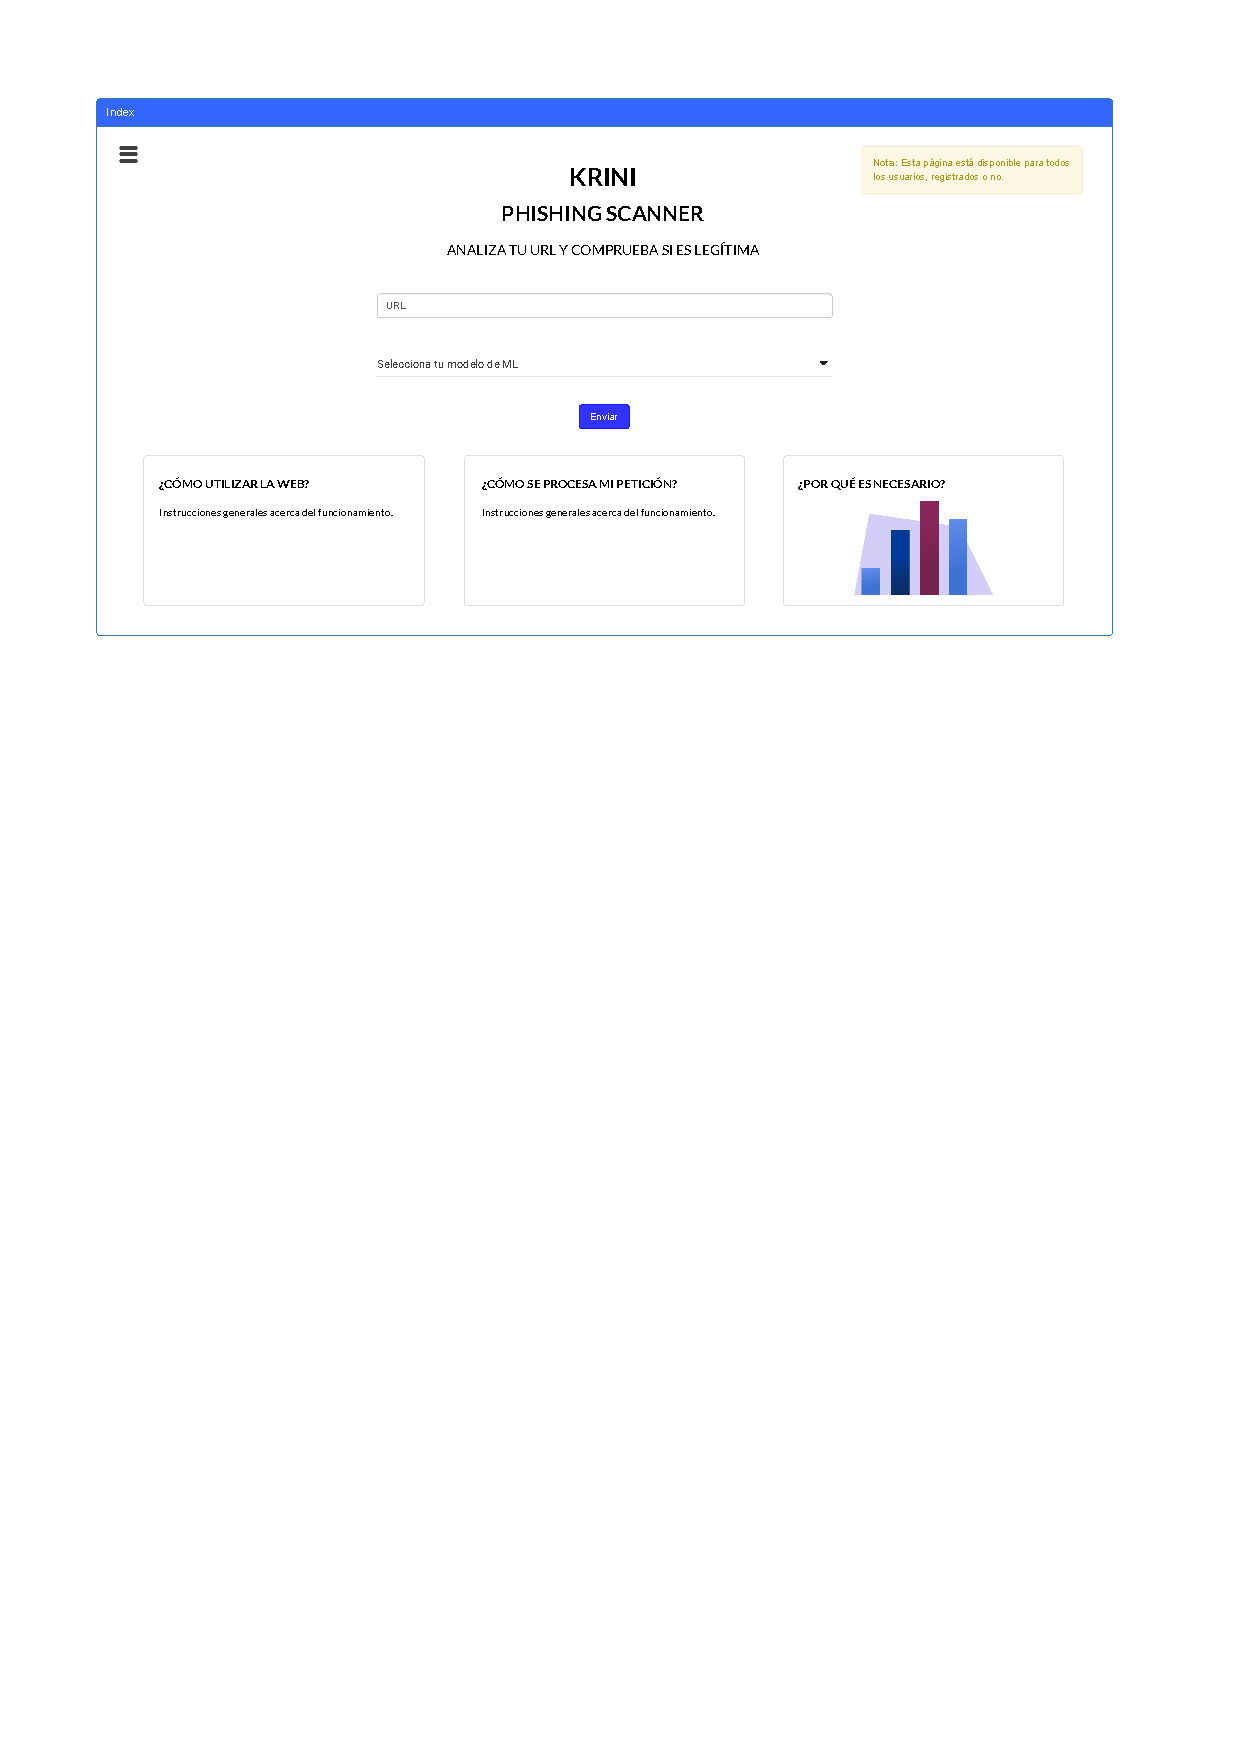
\includegraphics[width=\textwidth]{../img/anexos/mockups/1-mockups-index}
	\label{mock:index}
\end{figure}

\begin{figure}[h]
	\caption{Prototipos: \textit{dashboard}}
	\centering
	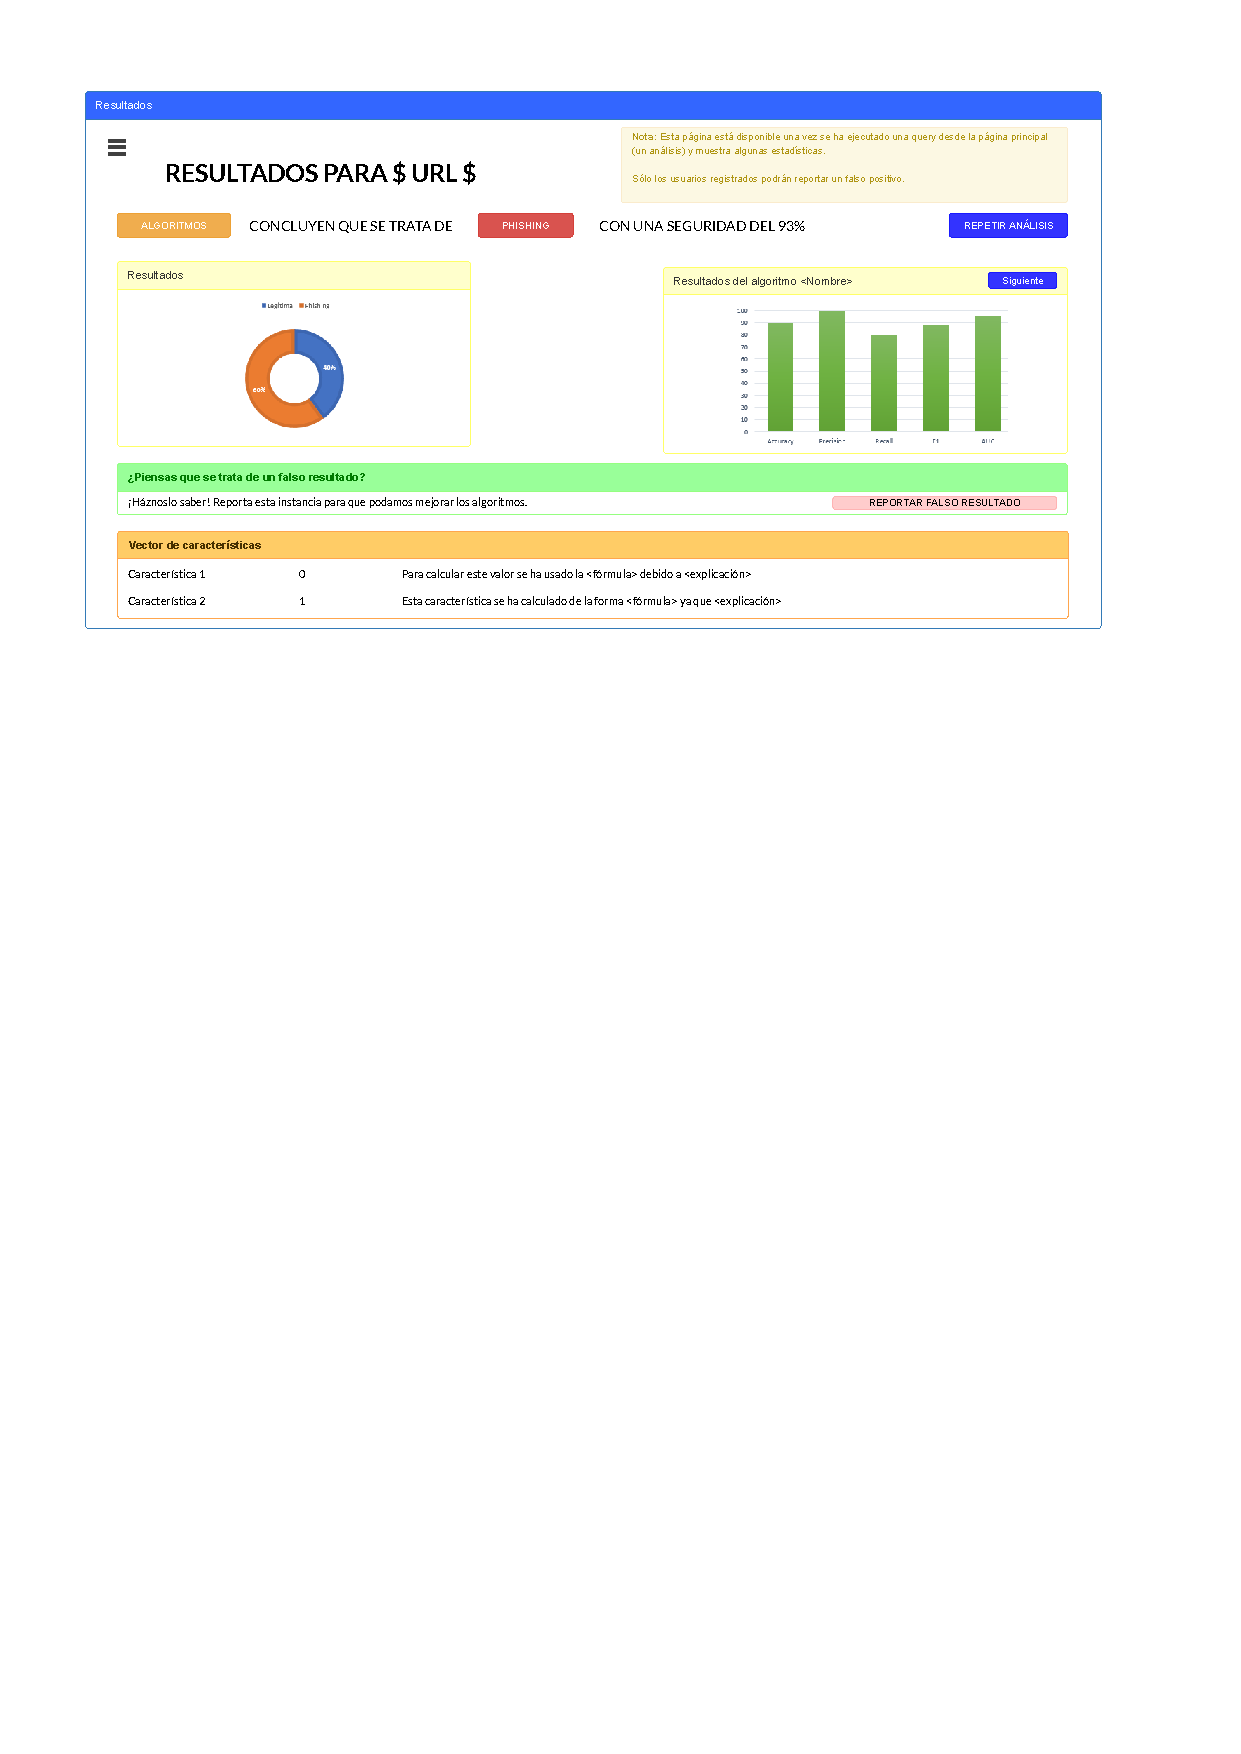
\includegraphics[width=\textwidth]{../img/anexos/mockups/2-mockups-dashboard}
	\label{mock:dashboard}
\end{figure}

\begin{figure}[h]
	\caption{Prototipos: reportar una URL}
	\centering
	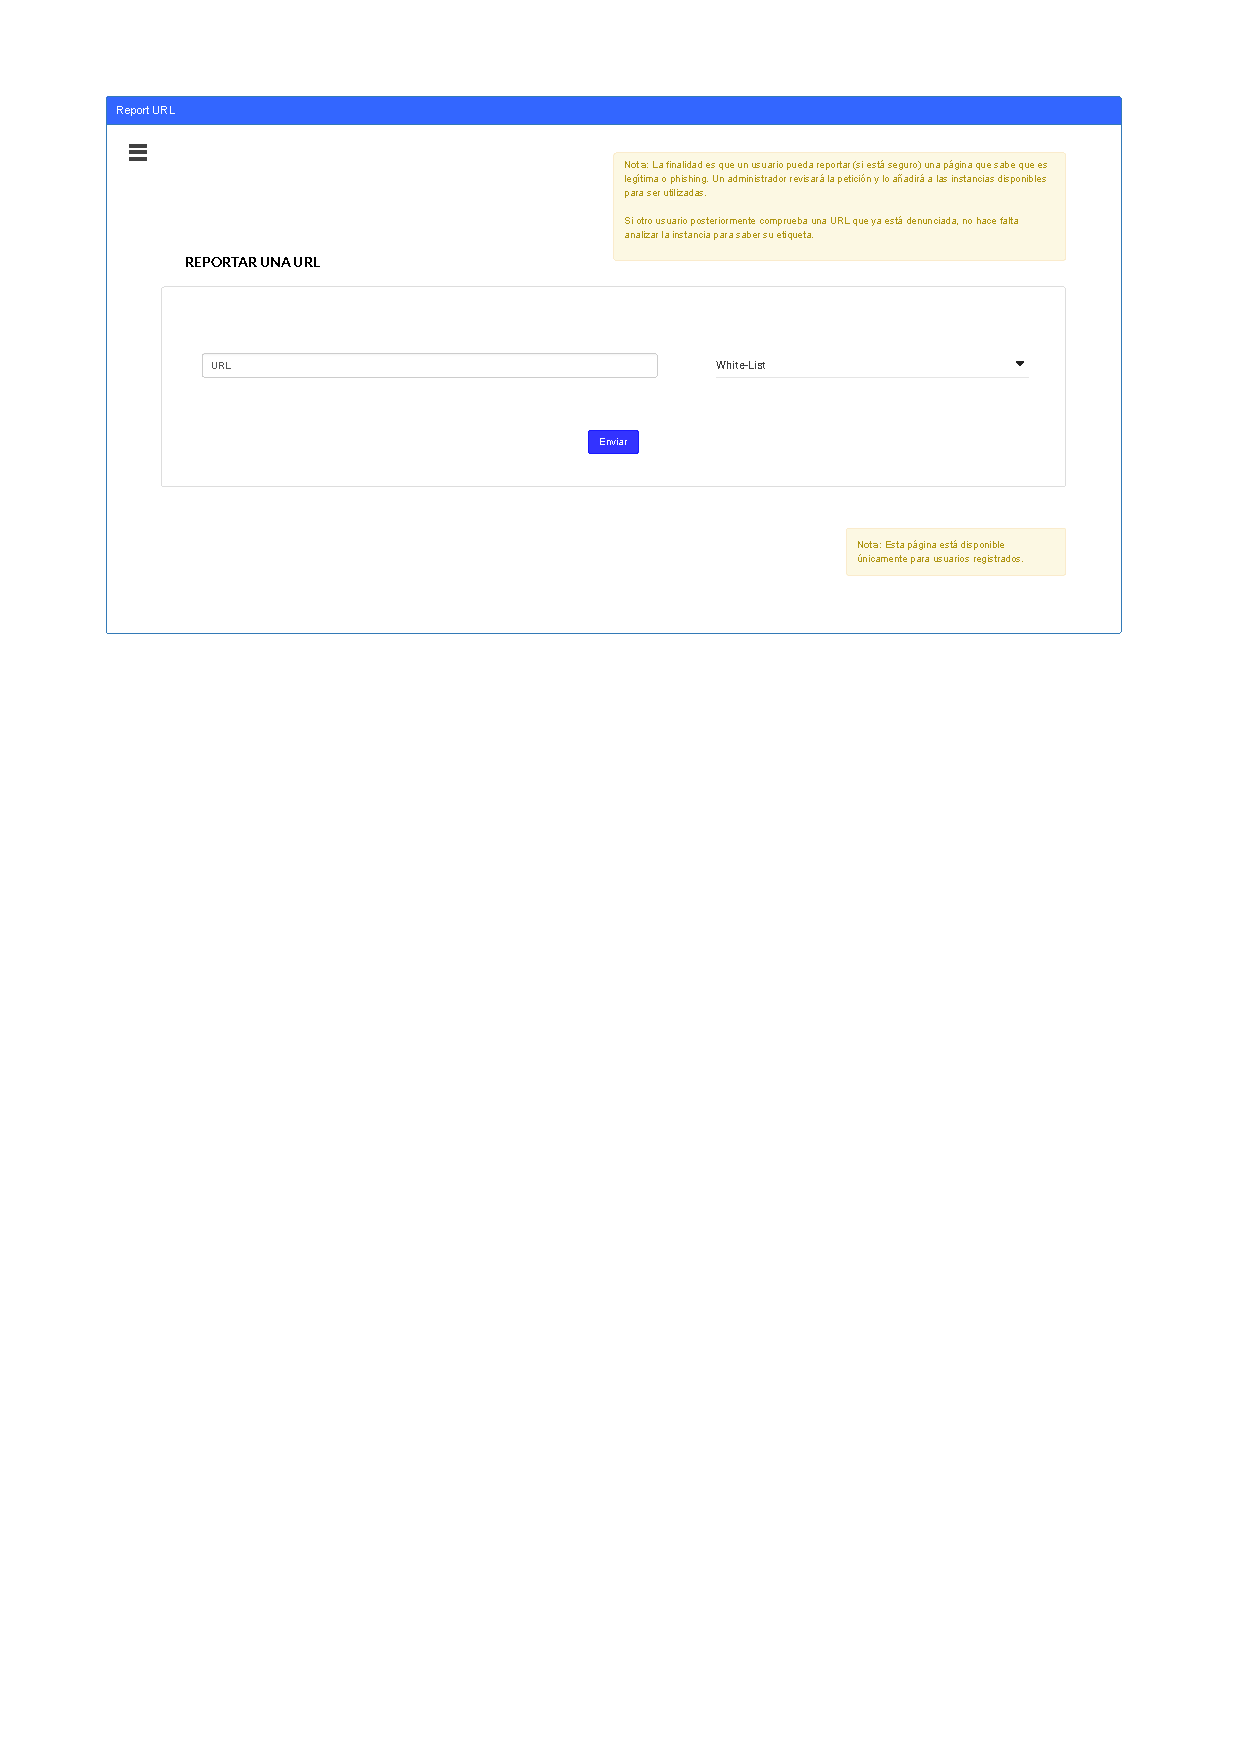
\includegraphics[width=\textwidth]{../img/anexos/mockups/3-mockups-report_url}
	\label{mock:report_url}
\end{figure}

\begin{figure}[h]
	\caption{Prototipos: perfil del usuario}
	\centering
	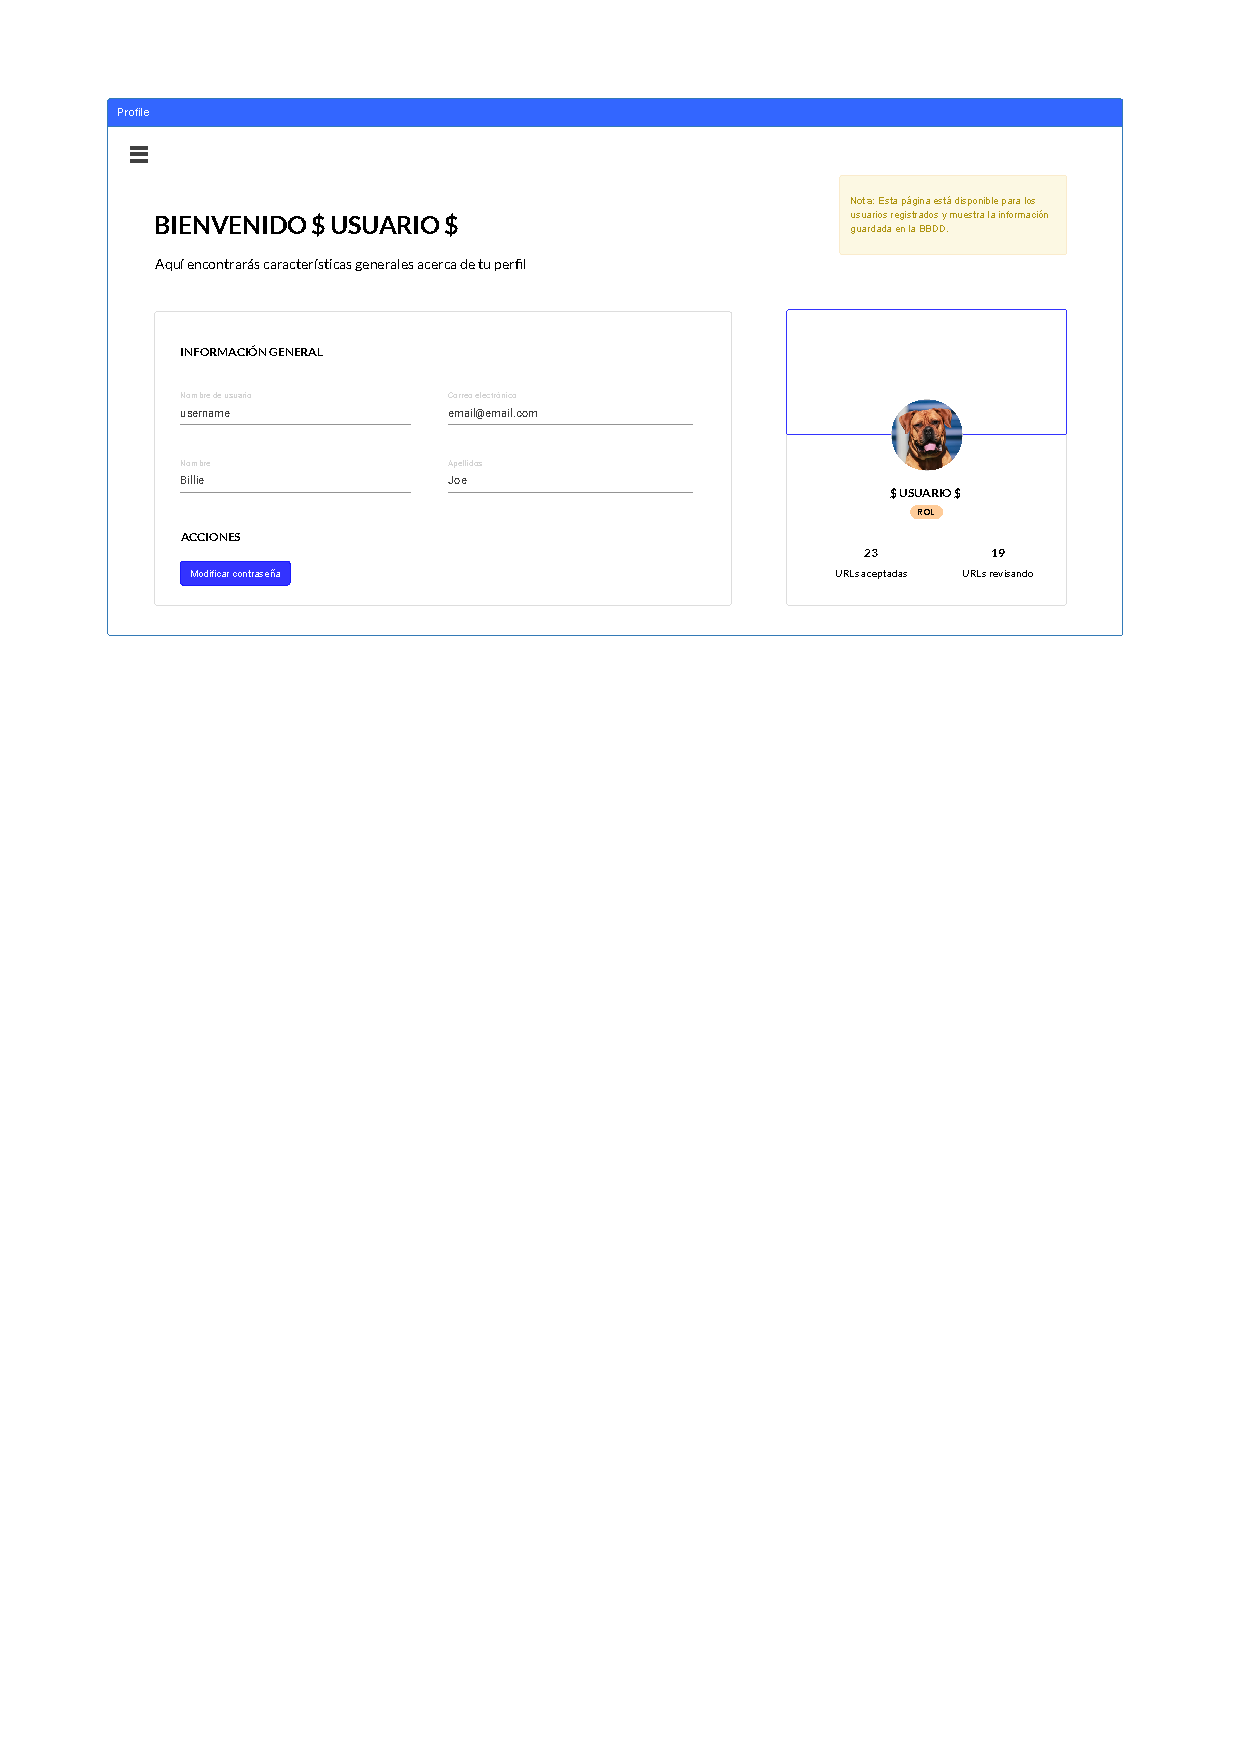
\includegraphics[width=\textwidth]{../img/anexos/mockups/4-mockups-profile}
	\label{mock:profile}
\end{figure}

\begin{figure}[h]
	\caption{Prototipos: administración de modelos}
	\centering
	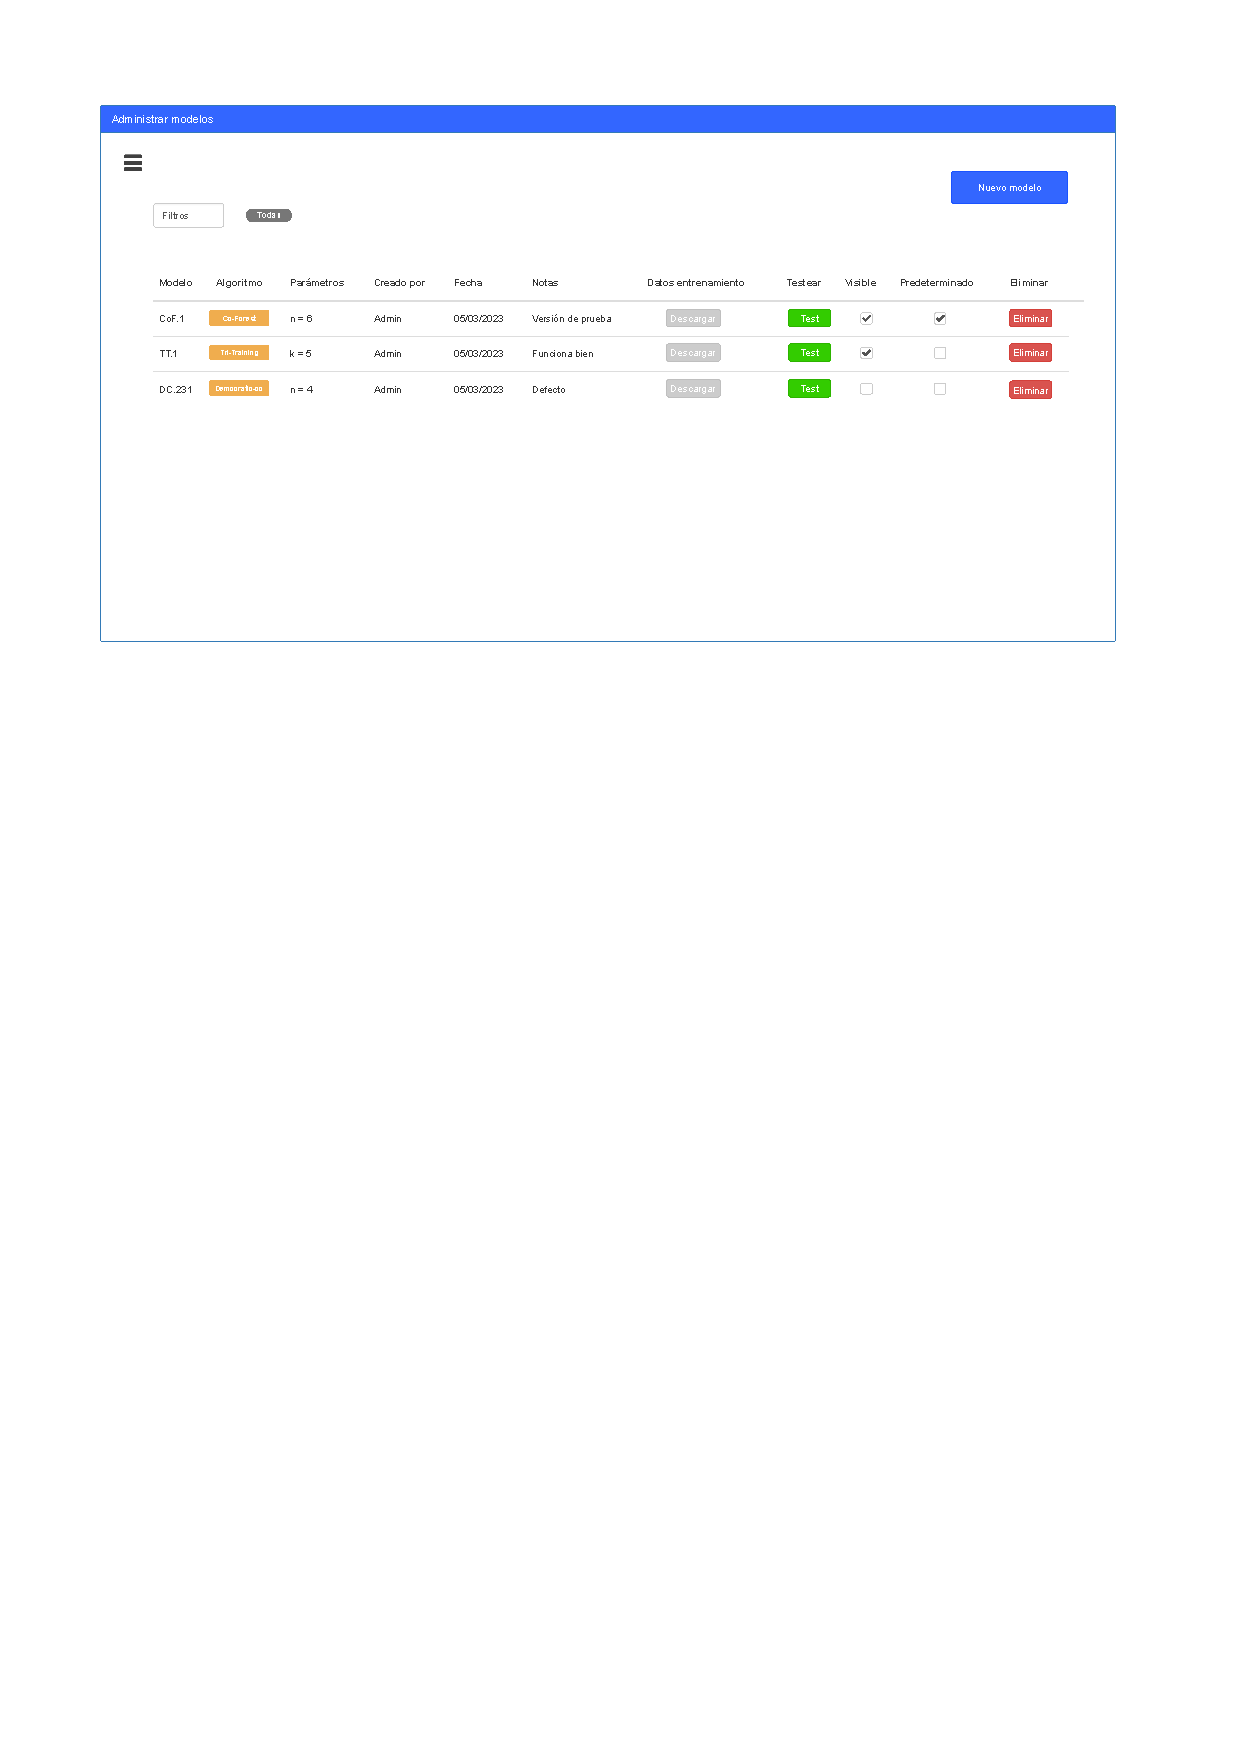
\includegraphics[width=\textwidth]{../img/anexos/mockups/5-mockups-models}
	\label{mock:model-admin}
\end{figure}

\begin{figure}[h]
	\caption{Prototipos: creación de modelos}
	\centering
	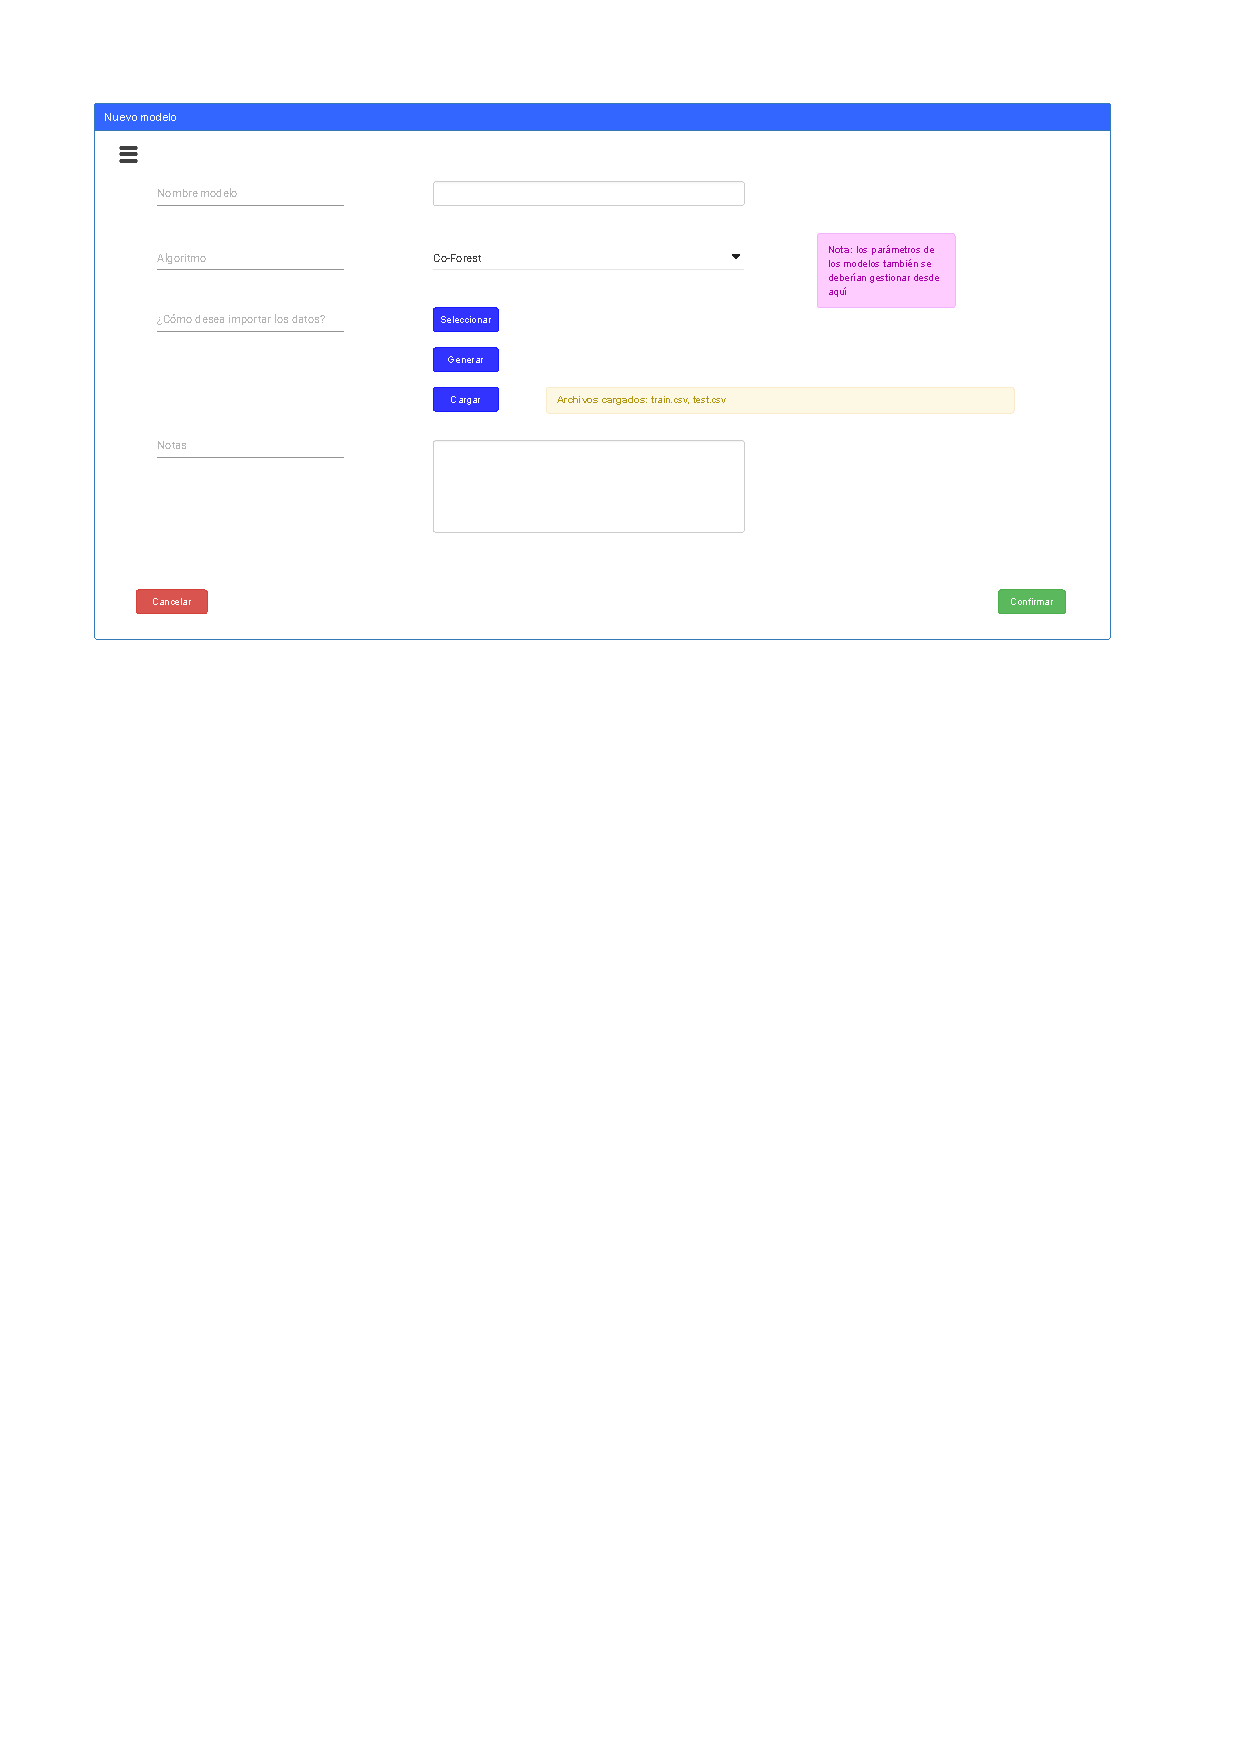
\includegraphics[width=\textwidth]{../img/anexos/mockups/6-mockups-new_model}
	\label{mock:model-new}
\end{figure}

\begin{figure}[h]
	\caption{Prototipos: evaluación de modelos}
	\centering
	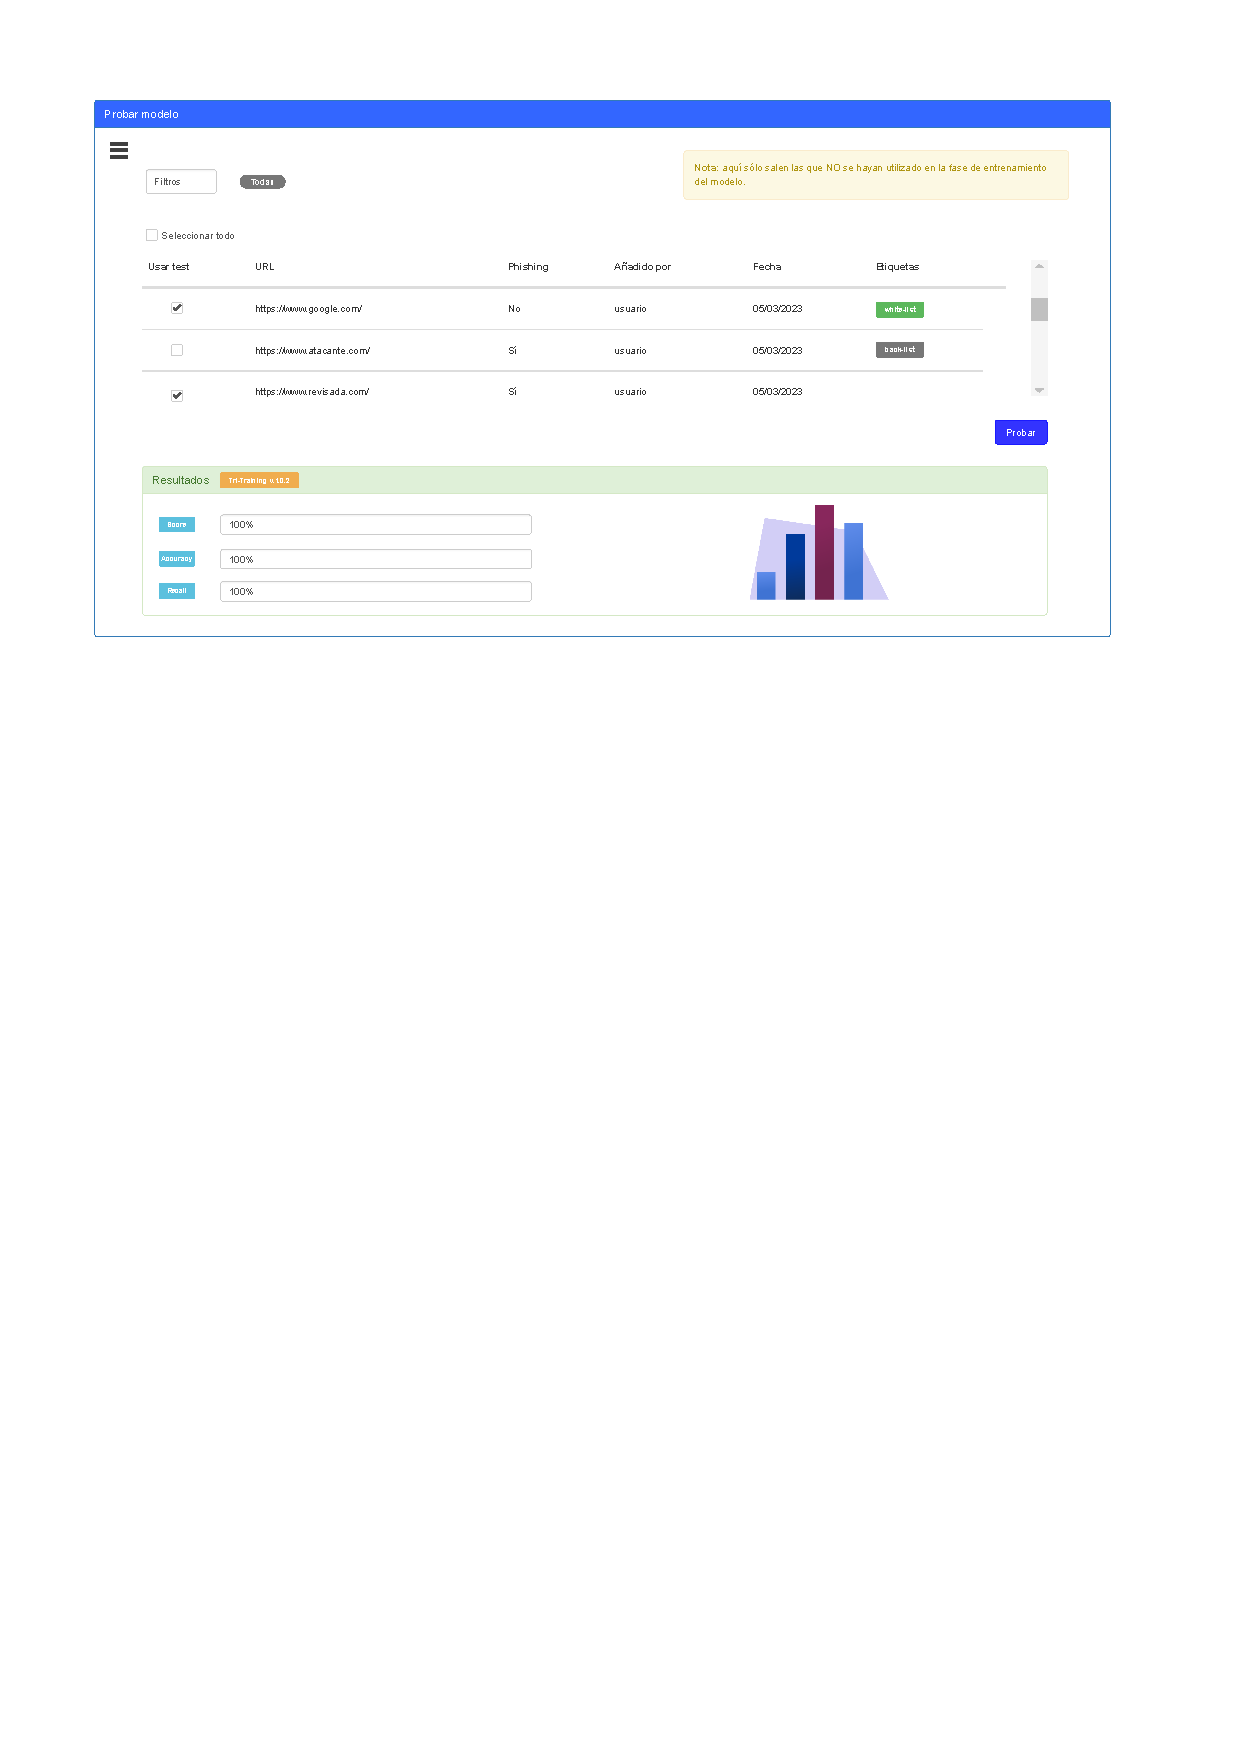
\includegraphics[width=\textwidth]{../img/anexos/mockups/7-mockups-test_model}
	\label{mock:model-test}
\end{figure}

\begin{figure}[h]
	\caption{Prototipos: selección de instancias}
	\centering
	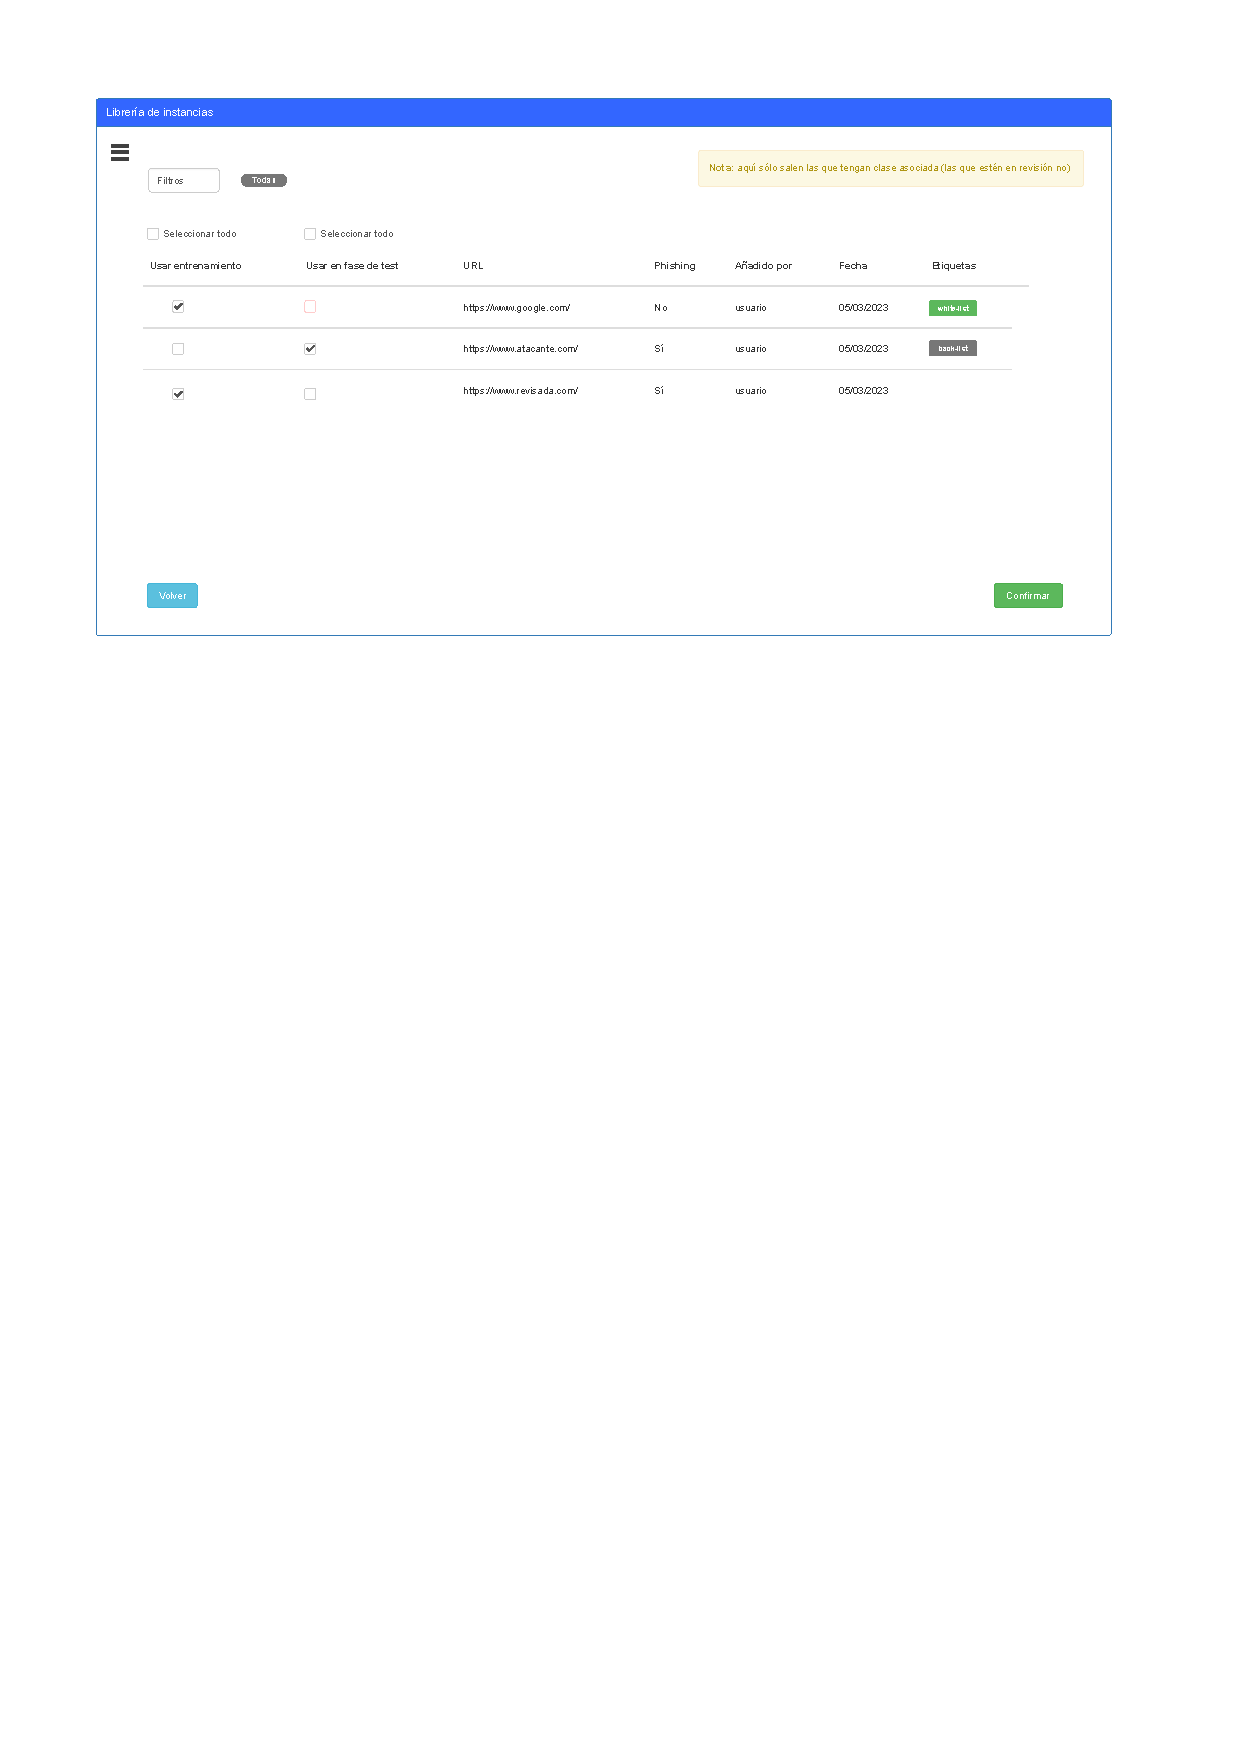
\includegraphics[width=\textwidth]{../img/anexos/mockups/8-mockups-select_instances}
	\label{mock:instance-selection}
\end{figure}

\begin{figure}[h]
	\caption{Prototipos: administración de instancias}
	\centering
	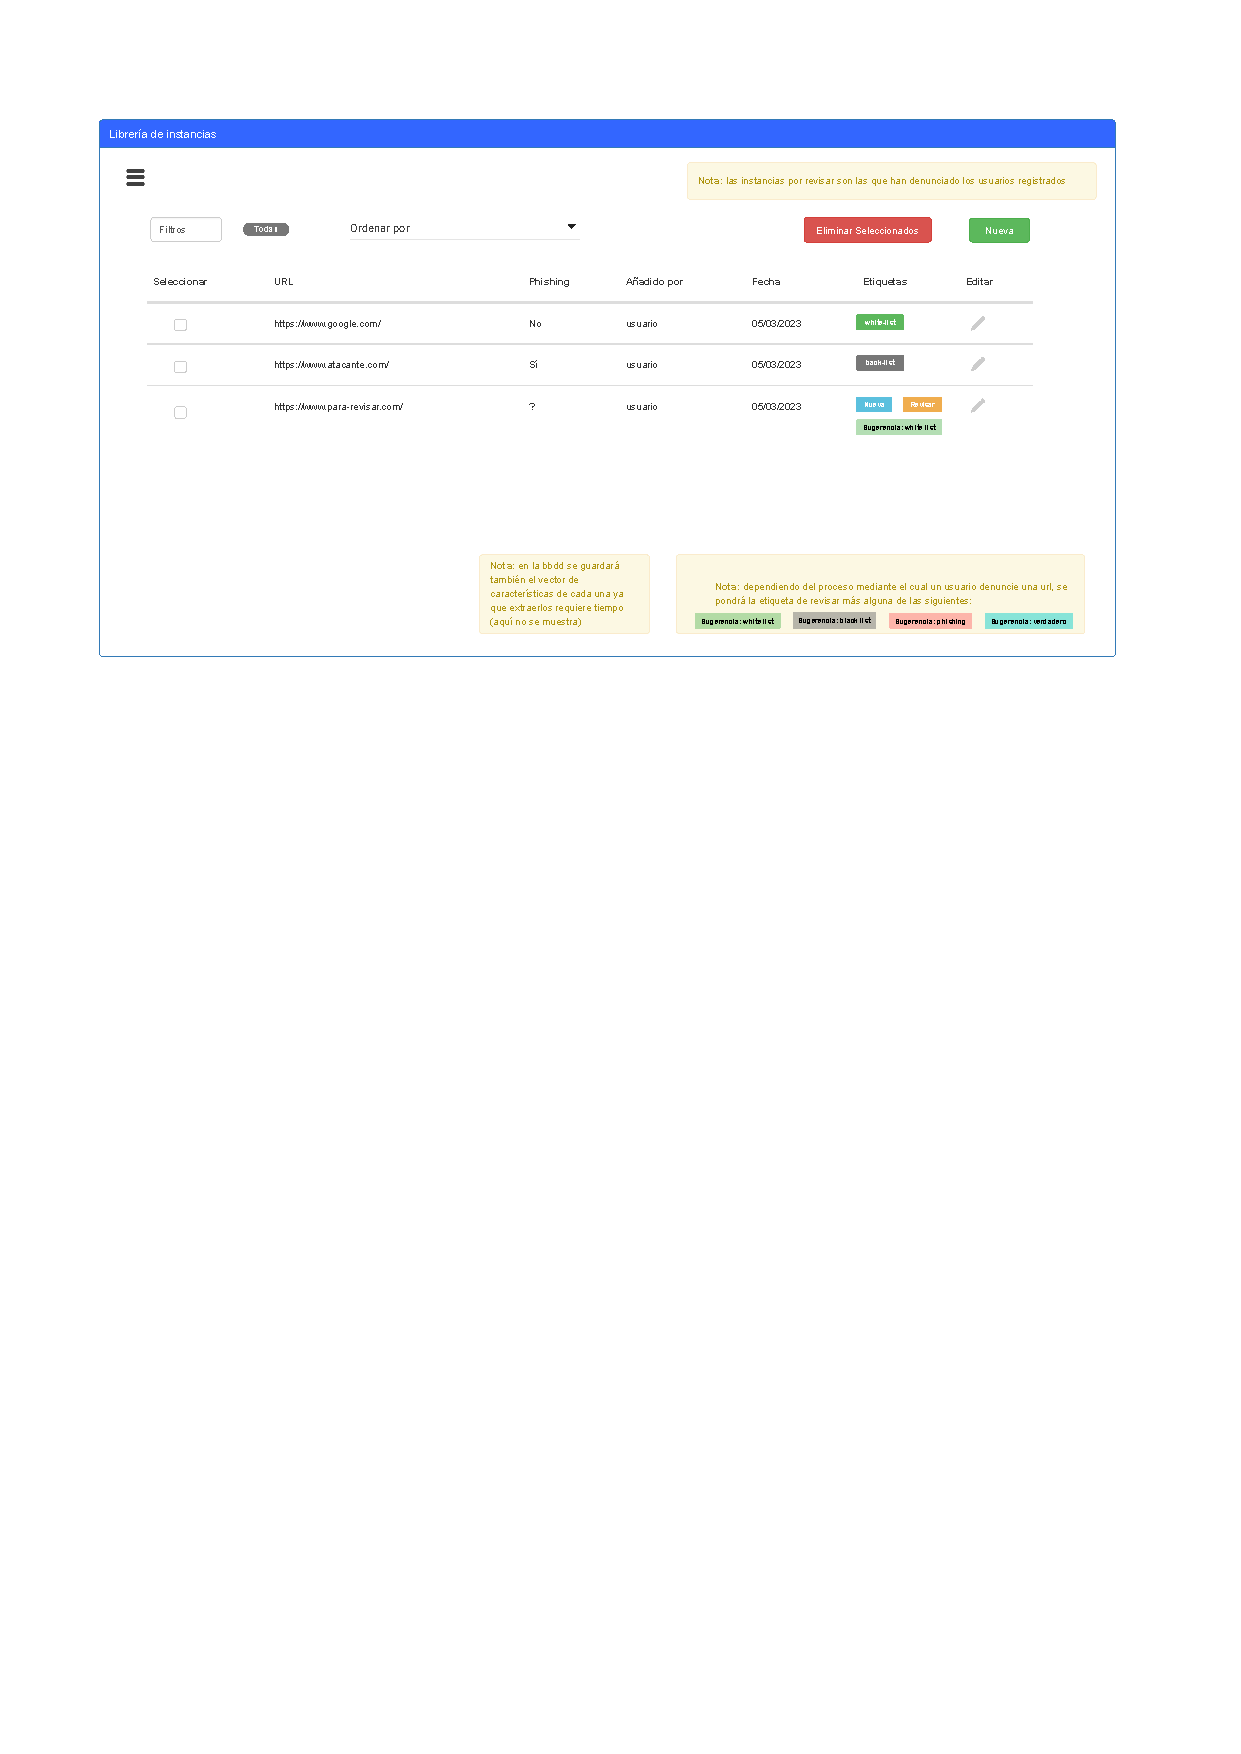
\includegraphics[width=\textwidth]{../img/anexos/mockups/9-mockups-instances}
	\label{mock:instance-admin}
\end{figure}

\begin{figure}[h]
	\caption{Prototipos: edición de instancias}
	\centering
	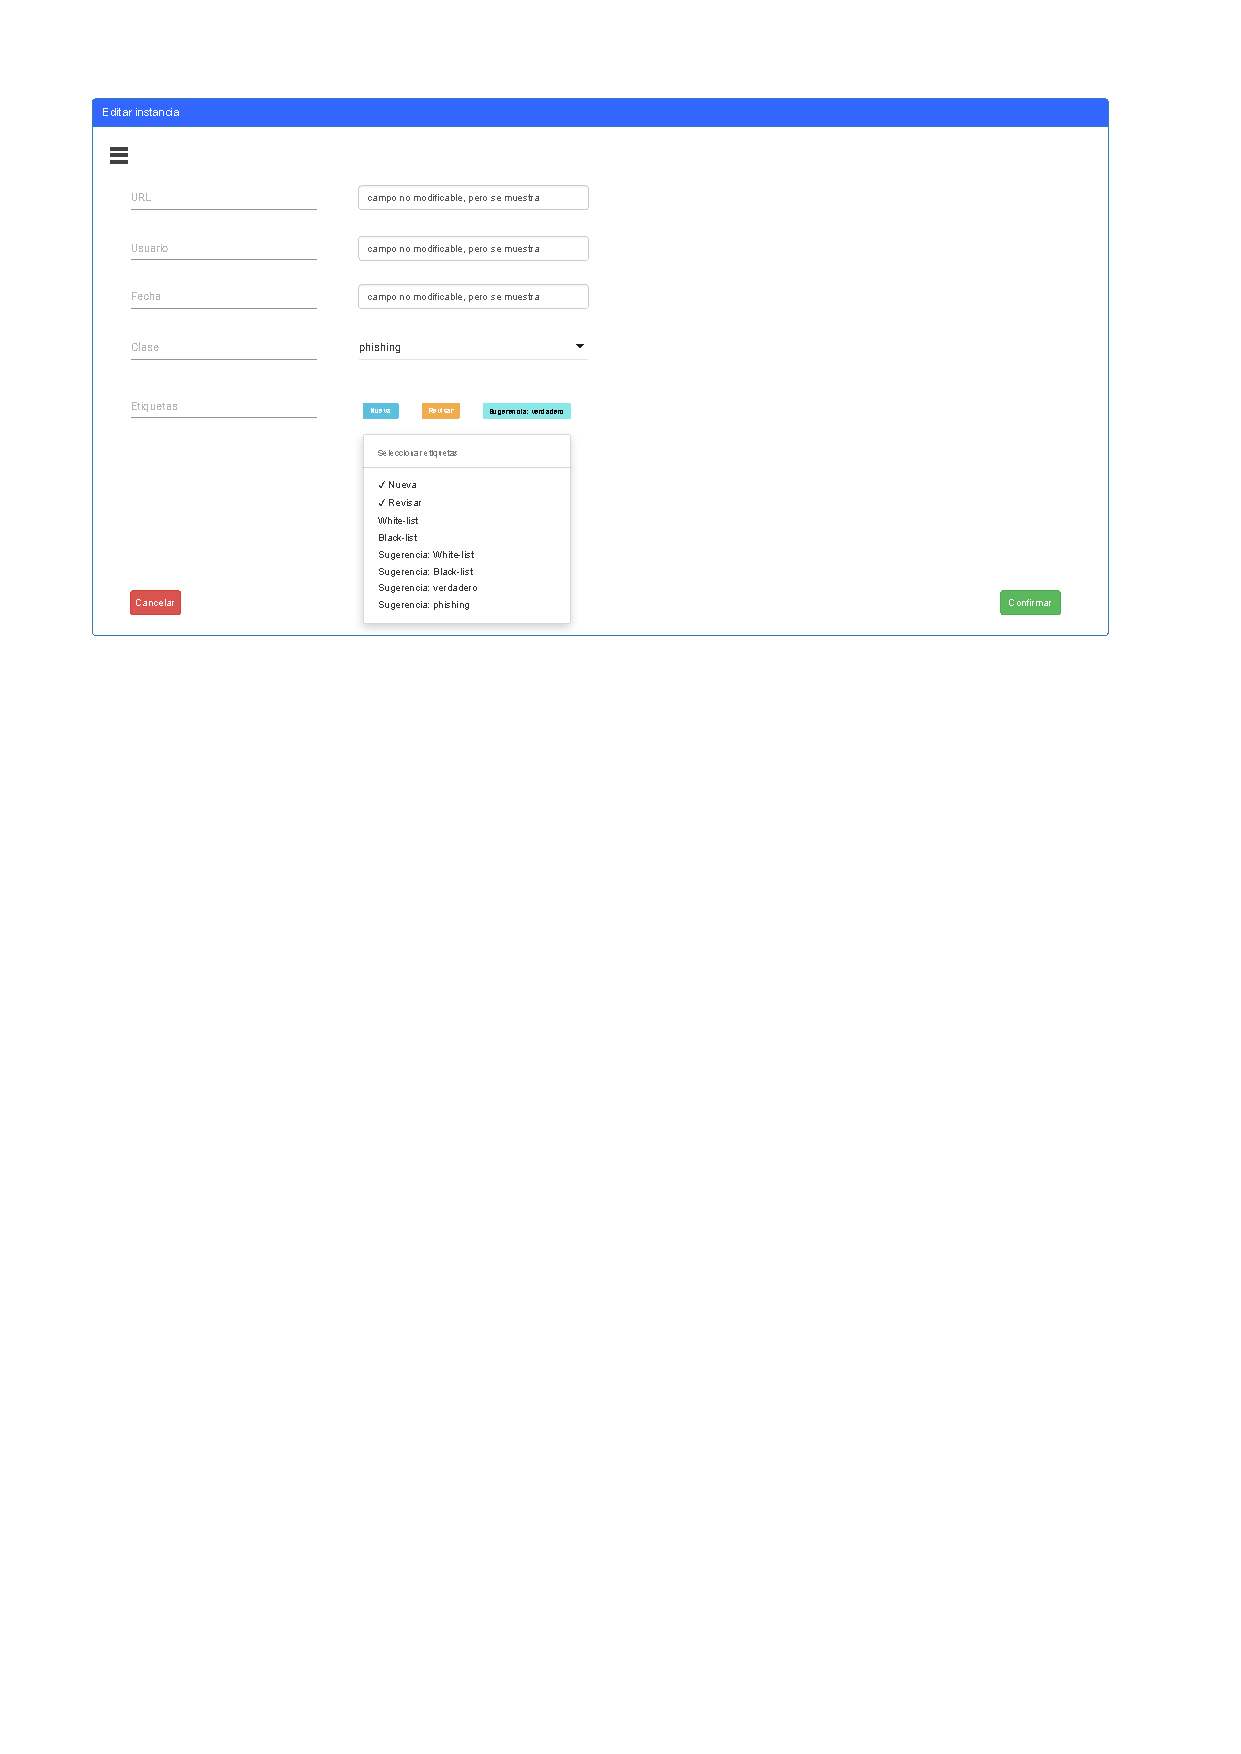
\includegraphics[width=\textwidth]{../img/anexos/mockups/10-mockups-edit_instance}
	\label{mock:instances-edit}
\end{figure}


\section{Especificación de requisitos}
\label{s:requisitos}

COMENTAR: Si estamos haciendo Scrum deberían ser historias de usuario (?)

Se detalla a continuación la especificación de requisitos de la aplicación \textit{web} propuesta.

\subsection{Diagrama de casos de uso}
\label{ss:diagrama-casos-uso}

Partiendo de las historias de usuario extraídas en las entrevistas realizadas con el \textit{product owner} y de los \textit{mockups} mostrados en la sección~\ref{ss:mockups}, se ha extraído el diagrama de casos de uso disponible en la figura~\ref{b:diagrama-cu}.

\begin{figure}[h]
	\caption{Diagramas: casos de uso}
	\centering
	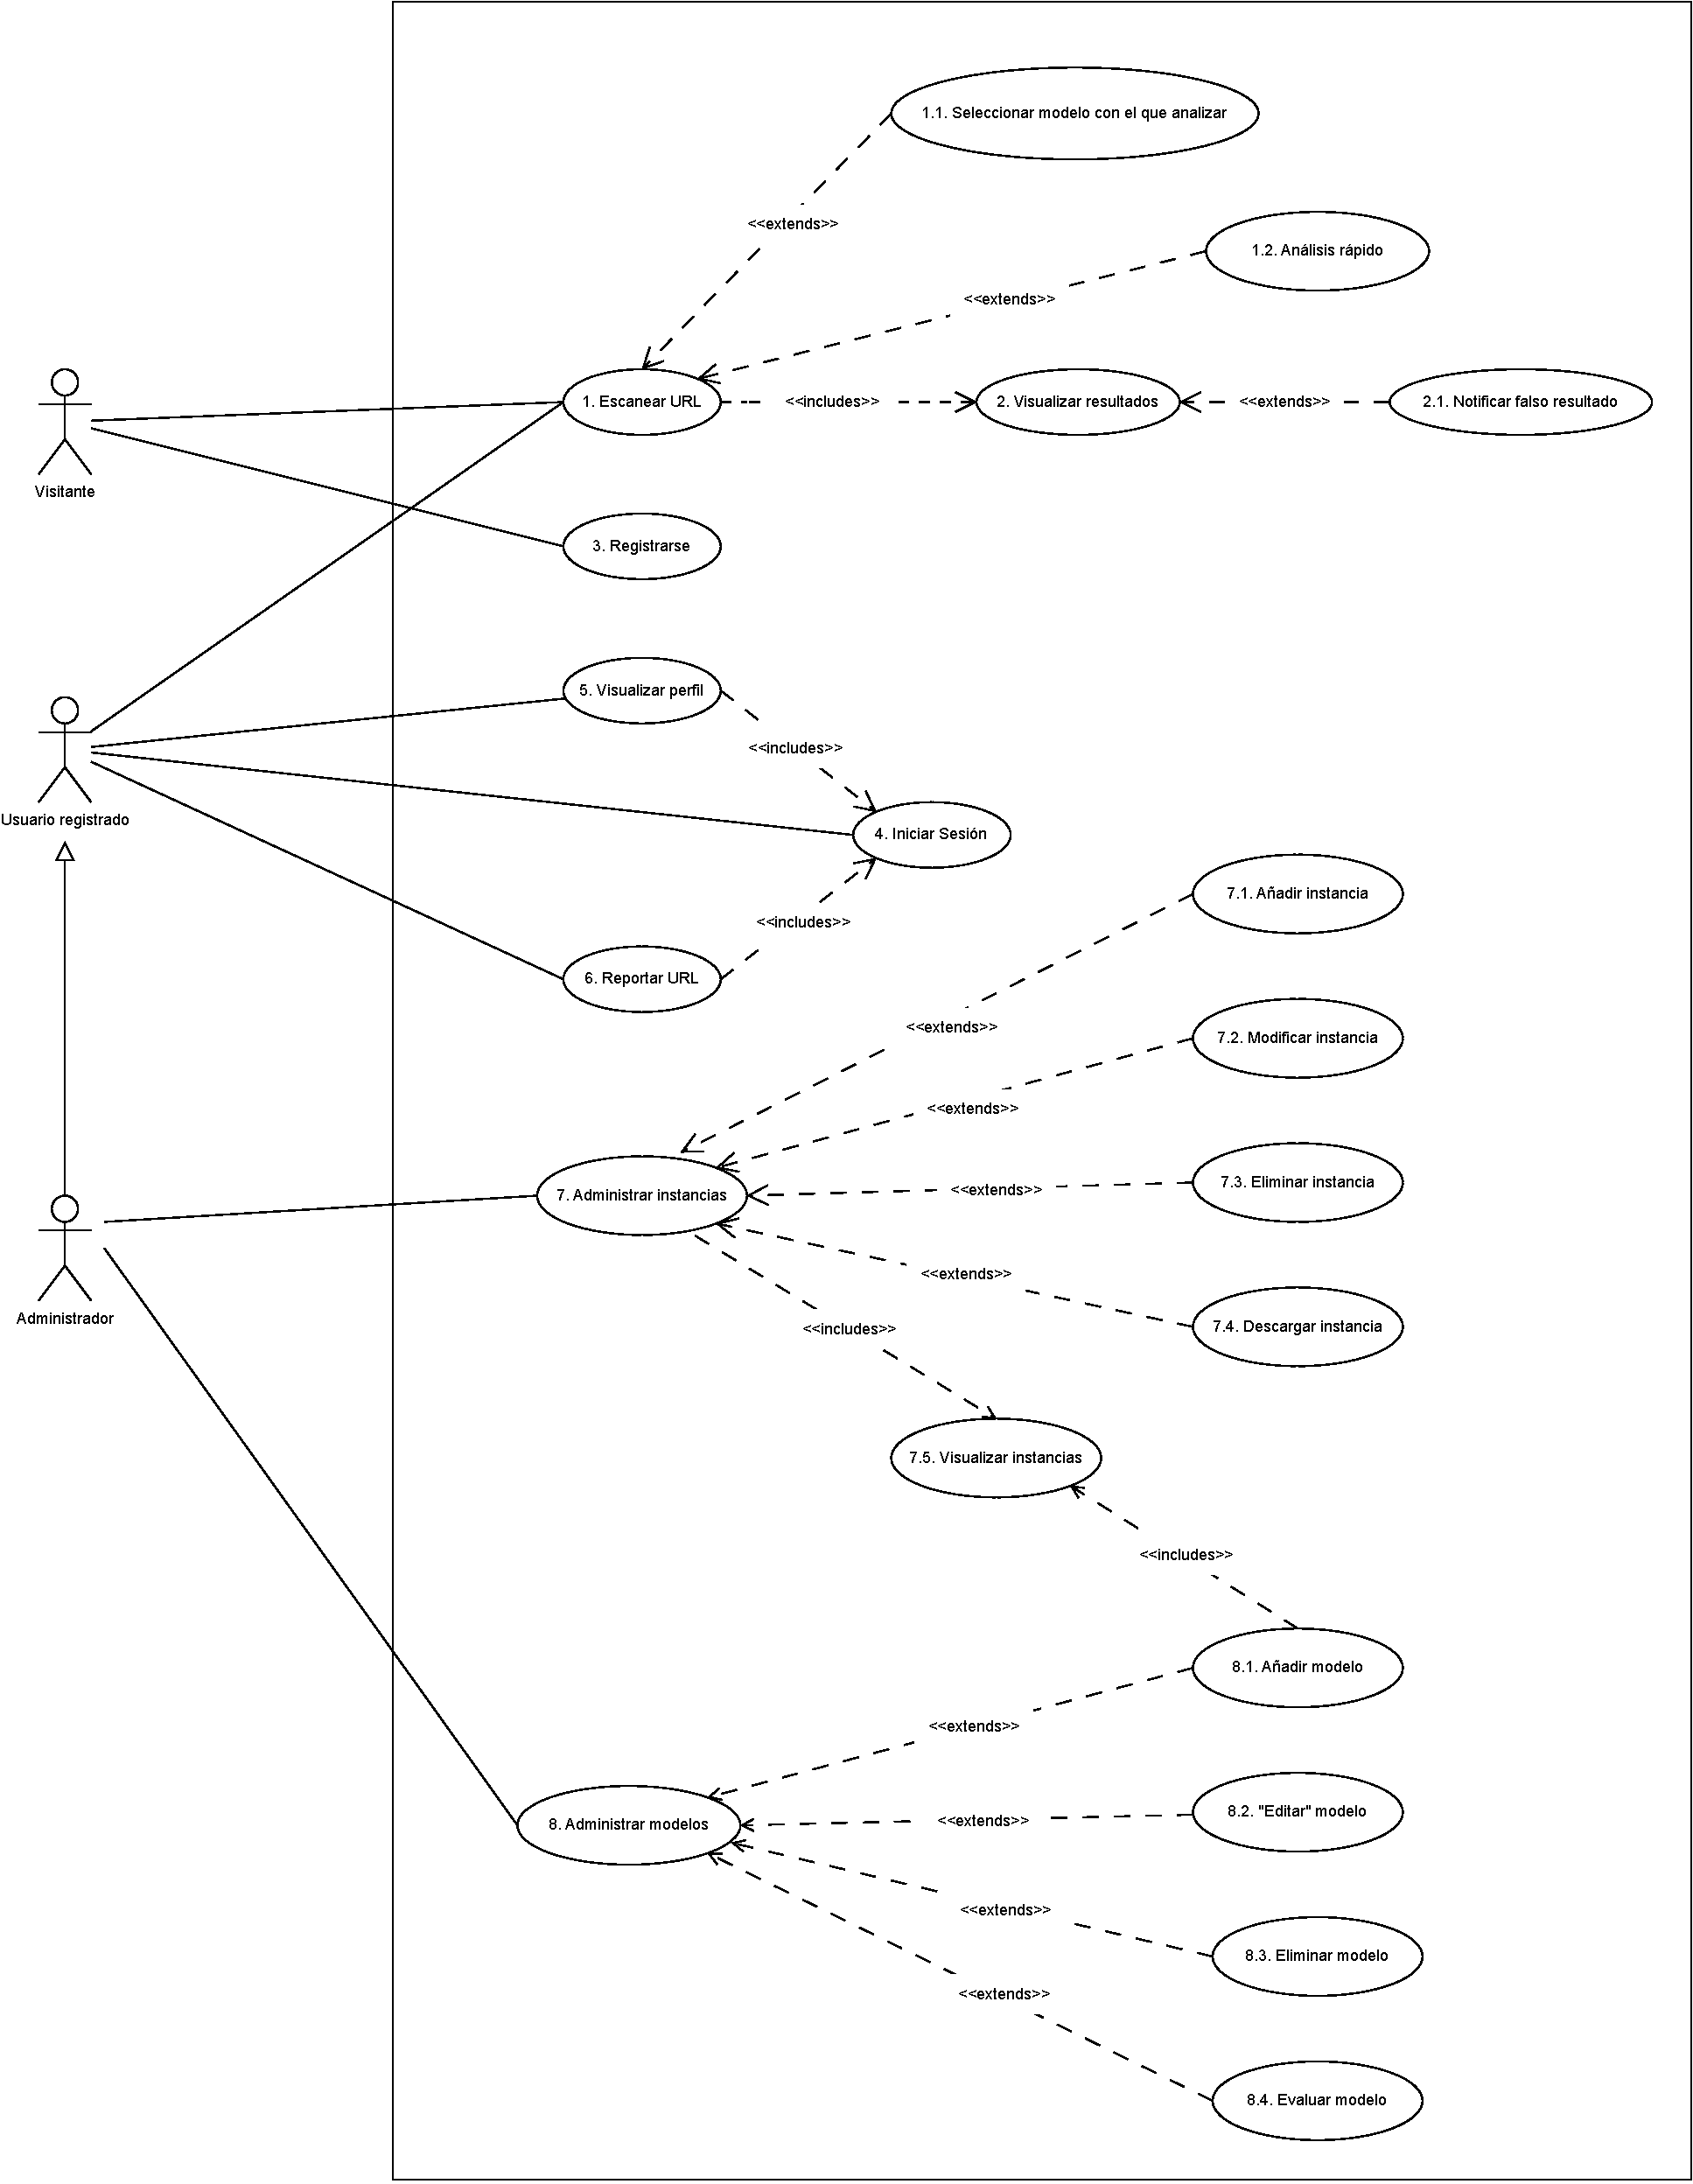
\includegraphics[width=\textwidth]{../img/anexos/diagrams/cu}
	\label{b:diagrama-cu}
\end{figure}

A continuación se muestra la tabla correspondiente a cada caso de uso.

% Caso de Uso 1 -> Escanear URL
\begin{table}[p]
	\centering
	\begin{tabularx}{\linewidth}{ p{0.21\columnwidth} p{0.71\columnwidth} }
		\toprule
		\textbf{CU-1}    & \textbf{Escanear URL}\\
		\toprule
		\textbf{Versión}              & 1.0    \\
		\textbf{Autor}                & Patricia Hernando Fernández \\
		\textbf{Requisitos asociados} & RF-xx, RF-xx \\
		\textbf{Descripción}          & Permitir que un usuario realice un escaneo de la URL que desee. Para ello, seleccionará los modelos que considere adecuados y se mostrarán los resultados en un \textit{dashboard} (CU-2 en la tabla~\ref{cu:visualizar-resultados}). \\
		\textbf{Precondición}         & No hay precondiciones. \\
		\textbf{Acciones}             &
		\begin{enumerate}
			\def\labelenumi{\arabic{enumi}.}
			\tightlist
			\item El usuario introduce la URL.
			\item El usuario selecciona los modelos de ML que considere (consultar CU-1.1 en la tabla~\ref{cu:seleccionar-modelos-ml}).
			\item El usuario decide si quiere realizar un análisis rápido.
			\item El usuario pulsa el botón de <<realizar análisis>>.
		\end{enumerate}\\
		\textbf{Postcondición}        & No hay postcondiciones. \\
		\textbf{Excepciones}          & En caso de que la URL introducida sea inalcanzable (tras aplicar reintentos) o que no haya ningún modelo disponible, el usuario será notificado y redirigido a la página principal. \\
		\textbf{Importancia}          & Alta \\
		\bottomrule
	\end{tabularx}
	\caption{CU-1 Escanear URL.}
	\label{cu:escanear-url}
\end{table}


% Caso de Uso 1.1 -> Seleccionar modelos
\begin{table}[p]
	\centering
	\begin{tabularx}{\linewidth}{ p{0.21\columnwidth} p{0.71\columnwidth} }
		\toprule
		\textbf{CU-1.1}    & \textbf{Seleccionar modelos con los que analizar}\\
		\toprule
		\textbf{Versión}              & 2.0    \\
		\textbf{Autor}                & Patricia Hernando Fernández \\
		\textbf{Requisitos asociados} & RF-xx, RF-xx \\
		\textbf{Descripción}          & Se mostrará al usuario los distintos modelos disponibles (y visibles) para que elija los que desee. \\
		\textbf{Precondición}         & Estar realizando el CU-1 (disponible en la tabla~\ref{cu:escanear-url}). \\
		\textbf{Acciones}             &
		\begin{enumerate}
			\def\labelenumi{\arabic{enumi}.}
			\tightlist
			\item Se cargan los modelos disponibles en la base de datos.
			\item El usuario selecciona los modelos que quiera utilizar.
		\end{enumerate}\\
		\textbf{Postcondición}        & Los modelos seleccionados quedan guardados. \\
		\textbf{Excepciones}          & En caso de no haber modelos disponibles la lista quedará vacía y se controlará la excepción en el CU-1 (tabla~\ref{cu:escanear-url}). \\
		\textbf{Importancia}          & Baja \\
		\bottomrule
	\end{tabularx}
	\caption{CU-1.1 Seleccionar modelos con los que analizar.}
	\label{cu:seleccionar-modelos-ml}
\end{table}

% Caso de Uso 2 -> Visualizar resultados
\begin{table}[p]
	\centering
	\begin{tabularx}{\linewidth}{ p{0.21\columnwidth} p{0.71\columnwidth} }
		\toprule
		\textbf{CU-2}    & \textbf{Visualizar resultados}\\
		\toprule
		\textbf{Versión}              & 1.0    \\
		\textbf{Autor}                & Patricia Hernando Fernández \\
		\textbf{Requisitos asociados} & RF-xx, RF-xx \\
		\textbf{Descripción}          & Se muestra al usuario los resultados tras haber analizado la URL mediante los algoritmos de ML seleccionados. Para ello se hará uso de un \textit{dashboard}, donde además se podrá notificar un falso resultado (CU-2.1 en la tabla~\ref{cu:notificar-falso-resultado}).\\
		\textbf{Precondición}         & Haber realizado un análisis previamente (CU-1 en la tabla~\ref{cu:escanear-url}). \\
		\textbf{Acciones}             &
		\begin{enumerate}
			\def\labelenumi{\arabic{enumi}.}
			\tightlist
			\item El usuario es redirigido a un \textit{dashboard}.
			\item El usuario puede interactuar con los distintos gráficos y la información mostrada en la página.
			\item El usuario puede notificar si considera que el análisis es erróneo (CU-2.1 en la tabla~\ref{cu:notificar-falso-resultado}).
		\end{enumerate}\\
		\textbf{Postcondición}        & No hay postcondiciones \\
		\textbf{Excepciones}          & En caso de intentar acceder al \textit{dashboard} sin haber realizado un análisis previo, el usuario será redirigido a la página principal con un mensaje informativo.\\
		\textbf{Importancia}          & Alta \\
		\bottomrule
	\end{tabularx}
	\caption{CU-2 Visualizar resultados.}
	\label{cu:visualizar-resultados}
\end{table}


% Caso de Uso 2.1 -> Notificar falso resultado
\begin{table}[p]
	\centering
	\begin{tabularx}{\linewidth}{ p{0.21\columnwidth} p{0.71\columnwidth} }
		\toprule
		\textbf{CU-2.1}    & \textbf{Notificar falso resultado}\\
		\toprule
		\textbf{Versión}              & 1.0    \\
		\textbf{Autor}                & Patricia Hernando Fernández \\
		\textbf{Requisitos asociados} & RF-xx, RF-xx \\
		\textbf{Descripción}          & Permite a un usuario notificar automáticamente a la aplicación si considera que el resultado de un análisis es erróneo.\\
		\textbf{Precondición}         & Encontrarse en el \textit{dashboard} tras un análisis (CU-2 en la tabla~\ref{cu:visualizar-resultados}) y haber iniciado sesión (CU-4 en la tabla~\ref{cu:iniciar-sesion}).\\
		\textbf{Acciones}             &
		\begin{enumerate}
			\def\labelenumi{\arabic{enumi}.}
			\tightlist
			\item El usuario pulsa el botón <<notificar falso resultado>>.
		\end{enumerate}\\
		\textbf{Postcondición}        & Se registra la URL notificada en la base de datos con el campo <<sugerencia>> establecido al valor opuesto del resultado mostrado. \\
		\textbf{Excepciones}          & Si el usuario no ha iniciado sesión, será informado de que la notificación no ha sido realizada por este motivo. En caso de errores con la base de datos se controlarán y se informará al usuario de la notificación no realizada.\\
		\textbf{Importancia}          & Baja \\
		\bottomrule
	\end{tabularx}
	\caption{CU-2.1  Notificar falso resultado.}
	\label{cu:notificar-falso-resultado}
\end{table}


% Caso de Uso 3 -> Registrarse
\begin{table}[p]
	\centering
	\begin{tabularx}{\linewidth}{ p{0.21\columnwidth} p{0.71\columnwidth} }
		\toprule
		\textbf{CU-3}    & \textbf{Registrarse}\\
		\toprule
		\textbf{Versión}              & 1.0    \\
		\textbf{Autor}                & Patricia Hernando Fernández \\
		\textbf{Requisitos asociados} & RF-xx, RF-xx \\
		\textbf{Descripción}          & Permite a un usuario crear una cuenta en la aplicación.\\
		\textbf{Precondición}         & El usuario no debe estar registrado ni haber iniciado sesión (CU-4 en la tabla~\ref{cu:iniciar-sesion}). \\
		\textbf{Acciones}             &
		\begin{enumerate}
			\def\labelenumi{\arabic{enumi}.}
			\tightlist
			\item El usuario selecciona <<Registrarse>>.
			\item El usuario introduce el nombre de usuario que considere.
			\item El usuario introduce un \textit{email} asociado a la cuenta.
			\item El usuario introduce la contraseña deseada.
			\item El usuario pulsa el botón de <<Registrar>>.
		\end{enumerate}\\
		\textbf{Postcondición}        & La información del nuevo usuario queda almacenada en la base de datos. \\
		\textbf{Excepciones}          & En caso de que los datos estén repetidos o el \textit{email} sea incorrecto, se pedirá al usuario que corrija los errores y no se creará la nueva cuenta. Si hay un usuario \textit{logueado} será redirigido a la página principal con un mensaje informativo.\\
		\textbf{Importancia}          & Media \\
		\bottomrule
	\end{tabularx}
	\caption{CU-3 Registrarse.}
	\label{cu:registrarse}
\end{table}


% Caso de Uso 4 -> Iniciar sesión
\begin{table}[p]
	\centering
	\begin{tabularx}{\linewidth}{ p{0.21\columnwidth} p{0.71\columnwidth} }
		\toprule
		\textbf{CU-4}    & \textbf{Iniciar sesión}\\
		\toprule
		\textbf{Versión}              & 1.0    \\
		\textbf{Autor}                & Patricia Hernando Fernández \\
		\textbf{Requisitos asociados} & RF-xx, RF-xx \\
		\textbf{Descripción}          & Permite a un usuario iniciar sesión en la aplicación.\\
		\textbf{Precondición}         & El usuario no debe haber iniciado sesión en el navegador (CU-4 en la tabla~\ref{cu:iniciar-sesion}). \\
		\textbf{Acciones}             &
		\begin{enumerate}
			\def\labelenumi{\arabic{enumi}.}
			\tightlist
			\item El usuario pulsa el botón de <<Iniciar sesión>>.
			\item El usuario introduce el nombre de usuario asociado a su cuenta.
			\item El usuario introduce la contraseña asociada a la cuenta.
			\item El usuario pulsa el botón de <<Iniciar sesión>>.
		\end{enumerate}\\
		\textbf{Postcondición}        & La información del usuario queda cargada en las variables de sesión. \\
		\textbf{Excepciones}          & En caso de que los datos sean incorrectos el usuario será notificado. Si hay un usuario \textit{logueado} será redirigido a la página principal con un mensaje informativo.\\
		\textbf{Importancia}          & Media \\
		\bottomrule
	\end{tabularx}
	\caption{CU-3 Iniciar sesión.}
	\label{cu:iniciar-sesion}
\end{table}

% Caso de Uso 5 -> Reportar URL
\begin{table}[p]
	\centering
	\begin{tabularx}{\linewidth}{ p{0.21\columnwidth} p{0.71\columnwidth} }
		\toprule
		\textbf{CU-5}    & \textbf{Reportar URL}\\
		\toprule
		\textbf{Versión}              & 1.0    \\
		\textbf{Autor}                & Patricia Hernando Fernández \\
		\textbf{Requisitos asociados} & RF-xx, RF-xx \\
		\textbf{Descripción}          & Permite a un usuario reportar una
		URL si considera que pertenece a una lista blanca o a una lista negra.\\
		\textbf{Precondición}         & El usuario debe de haber iniciado sesión (CU-4 en la tabla~\ref{cu:iniciar-sesion}). \\
		\textbf{Acciones}             &
		\begin{enumerate}
			\def\labelenumi{\arabic{enumi}.}
			\tightlist
			\item El usuario introduce la URL a reportar.
			\item El usuario selecciona el tipo de lista a la que pertenece la URL.
			\item El usuario pulsa el botón de <<Enviar>>.
		\end{enumerate}\\
		\textbf{Postcondición}        & Se registra la URL reportada en la base de datos con el campo <<sugerencia>> establecido al valor seleccionado en el desplegable (ejemplo: \textit{white-list}). \\
		\textbf{Excepciones}          & En caso de no haber iniciado sesión, el usuario será redirigido a una pantalla especial (error 403, acceso restringido) con un enlace para iniciar sesión. Se controla en aplicación que el usuario haya rellenado todos los campos necesarios. \\
		\textbf{Importancia}          & Baja \\
		\bottomrule
	\end{tabularx}
	\caption{CU-5 Reportar URL.}
	\label{cu:reportar-url}
\end{table}


